\chapter{Studi Literatur}

Pada bab ini,  diisi oleh studi literatur, hal-hal yang berkaitan dengan topik persoalan tugas akhir  dipaparkan dalam bab ini untuk memberikan informasi mengenai dasar teori dan studi yang dipakai. Bab ini diharapkan membantu pembaca untuk mengerti dalam membaca penelitian tugas akhir ini.

\section{\textit{Natural Language Processing}}

Pemrosesan Bahasa Alami (PBA) atau dalam bahasa Inggris dikenal dengan \textit{Natural Language Processing} (NLP) merupakan cabang dari ilmu komputer, kecerdasan buatan, dan linguistik yang berfokus pada interaksi antara komputer dan bahasa manusia. NLP bertujuan untuk memungkinkan komputer tidak hanya memahami dan menafsirkan bahasa manusia, tetapi juga menghasilkannya dengan cara yang bermakna dan efektif. Hal ini dijelaskan oleh \citeauthor{nlp} \parencite{nlp}, yang menyatakan pentingnya NLP dalam membangun jembatan komunikasi antara manusia dan mesin.

Dalam beberapa dekade terakhir, NLP telah mengalami kemajuan yang signifikan, memungkinkan komputer tidak hanya memahami bahasa manusia tetapi juga merespons dengan cara yang semakin kompleks dan kontekstual. Teknologi seperti mesin penerjemah, asisten virtual, dan sistem rekomendasi semuanya memanfaatkan prinsip-prinsip NLP untuk berfungsi \parencite{nlp}.

Salah satu tantangan utama dalam NLP adalah keragaman dan kompleksitas bahasa manusia. Bahasa penuh dengan nuansa, ambiguitas, dan struktur yang dapat bervariasi tergantung pada konteks dan budaya \parencite{ai}. Untuk mengatasi tantangan ini, berbagai tugas NLP telah didefinisikan dan dikembangkan untuk memecahkan masalah pemahaman bahasa menjadi komponen yang lebih kecil dan lebih spesifik.

Beberapa tugas NLP yang dibahas pada studi literatur adalah, \textit{Named Entity Recognition} (NER), \textit{Sentiment Analysis}, dan \textit{Summarization}. Masing-masing tugas ini menargetkan aspek tertentu dari pemahaman bahasa dan memiliki aplikasi praktisnya sendiri dalam berbagai bidang, mulai dari analisis teks hingga pengembangan sistem percakapan otomatis.

\subsection{\textit{Named-Entity Recognition} (NER)}

NER merupakan salah satu tugas dari NLP yang bertujuan untuk mengklasifikasikan entitas pada sebuah teks \parencite{ner}. Setiap entitas yang ada pada sebuah teks akan diklasifikasikan menjadi sebuah label. Label ini tergantung pada \textit{dataset} yang digunakan.

\begin{table}[h]
    \vspace{0.25cm}
    \caption{Contoh Data NER \parencite{ner}}
    \label{table:contoh-data-ner}
    \begin{center}
        \begin{tabular}{cll}
            \hline
            \textbf{Label} & \textbf{Informasi} & \textbf{Contoh} \\ \hline
            PER & Nama orang & Joko Widodo, Soekarno \\ \hline
            LOC & Nama lokasi & Indonesia, Bandung \\ \hline
            ORG & Nama organisasi & Telkom, DPR \\ \hline
        \end{tabular}
    \end{center}
\end{table}

Pada penelitian yang dilakukan oleh \citeauthor{ner}, dilakukan NER pada \textit{dataset} yang berisi \textit{tweet} berbahasa Indonesia. Sebagai contoh yang bisa dilihat pada tabel \ref{table:contoh-data-ner}, "Soekarno" dan "Joko Widodo" dapat dikenali sebagai nama orang dengan label PER dalam sebuah kalimat "Soekarno dan Joko Widodo merupakan presiden Indonesia". 

Selain diklasifikasikan menjadi label saja, data juga menggunakan format BIO (\textit{Begin, Inside}, dan \textit{Other}). Label B-XXX akan menyatakan kata pertama dan I-XXX menyatakan kata selanjutnya pada suatu entitas XXX. Sedangkan, O digunakan sebagai kata yang ada di luar entitas atau label yang disediakan pada \textit{dataset} \parencite{ner}. Tabel \ref{table:contoh-labeling-ner} merupakan contoh \textit{labeling} yang mengandung nama organisasi (ORG, Telkom University), nama orang (PER, Ridwan Kamil), dan nama lokasi (LOC, Bandung).

\begin{table}[h]
    \vspace{0.25cm}
    \caption{Contoh \textit{Labeling} NER \parencite{ner}}
    \label{table:contoh-labeling-ner}
    \begin{center}
        \begin{tabular}{ll}
            \hline
            \textbf{Data} & \textbf{NER Label} \\ \hline
            @infobdg & O \\ \hline
            Ridwan & B-PER \\ \hline
            Kamil & I-PER \\ \hline
            berkunjung & O \\ \hline
            ke & O \\ \hline
            Telkom & B-ORG \\ \hline
            University & I-ORG \\ \hline
            yang & O \\ \hline
            terletak & O \\ \hline
            di & O \\ \hline
            Bandung & B-LOC \\ \hline
        \end{tabular}
    \end{center}
\end{table}

\subsection{\textit{Sentiment Analysis}}

\textit{Sentiment analysis} merupakan proses untuk mengklasifikasikan polaritas dari sebuah opini. Opini dalam konteks NLP berupa sebuah teks \parencite{sentiment_stock}. Terdapat banyak klasifikasi dari sentimen, salah satunya adalah klasifikasi sentimen ke dalam 3 kelas yaitu positif, negatif, dan netral. Teks yang mengandung kata-kata dengan sentimen positif seperti baik, hebat, lezat, dan lain-lain akan diklasifikasikan sebagai positif, begitu pula sebaliknya. Sedangkan, kata-kata yang tidak mengandung sentimen positif maupun negatif akan diklasifikasikan sebagai netral.

Terdapat tiga tingkat klasifikasi utama pada \textit{sentiment analysis} yaitu tingkat dokumen, kalimat, dan aspek \parencite{sentiment_algo}. \textit{Sentiment analysis} tingkat dokumen bertujuan untuk mengklasifikasikan sebuah dokumen yang mengandung opini tertentu, tingkat dokumen akan memperhatikan seluruh dokumen untuk menentukan sentimennya. Tingkat kalimat akan mempertimbangkan sentimen pada tingkat kalimat. Sedangkan, pada tingkat aspek akan hanya mempertimbangkan pada suatu aspek atau entitas saja.

\subsection{\textit{Summarization}}

\textit{Summarization} mempunyai tujuan untuk menghasilkan ringkasan dari serangkaian teks atau dokumen \parencite{summarization}. Hasil ringkasan harus mempertahankan informasi penting dengan panjang yang lebih sedikit dibandingkan dengan teks atau dokumen aslinya. Terdapat dua jenis \textit{summarization} tergantung dari cara mendapatkannya, yaitu \textit{extractive} dan \textit{abstractive}. \textit{Extractive summarization} akan mengekstrak kata demi kata yang penting dari dokumen aslinya. Sebaliknya, \textit{abstractive summarization} berusaha menghasilkan abstrak yang mungkin mengandung kata yang tidak terdapat pada dokumen aslinya \parencite{summarization}.


\begin{table}[h]
    \vspace{0.25cm}
    \caption{Contoh Data \textit{Summarization} \parencite{summarization}}
    \label{table:contoh-data-summ}
    \begin{center}
        \begin{tabularx}{\textwidth}{X}
            \hline
            \textbf{Dokumen} \\ \hline
            \uwave{\textbf{Suara.com = Cerita sekuel terbaru James Bond bocor}} \\
            \uwave{Menurut sumber yang terlibat dalam produksi film ini, agen rahasia 007 berhenti menjadi mata-mata Inggris demi menikah dengan perempuan yang dicintainya.} \\
            "Bond berhenti menjadi agen rahasia karena jatuh cinta dan menikah dengan perempuan yang dicintai", tutur seorang sumber yang dekat dengan produksi seperti dikutip laman PageSix.com. \\
            Dalam film tersebut, Bond diduga menikahi Madelein Swann yang diperankan oleh Lea Seydoux. \\
            Lea diketahui bermain sebagai gadis Bond di sekuel Spectre pada 2015 silam. \\
            \uwave{Jika benar, ini merupakan satu-satunya sekuel yang bercerita pernikahan James Bond sejak 1969.} \\
            \uwave{Sebelumnya, di sekuel On Her Majesty, James Bond menikahi Tracy Draco yang diperankan Diana Rigg.} \\
            \uwave{Namun, di film itu Draco terbunuh.} \\
            Plot sekuel film James Bond ke-25 bocor tak lama setelah Daniel Craig mengumumkan bakal kembali memerankan tokoh agen 007. \\ \hline
            \textbf{Ringkasan} \\ \hline
            Cerita sekuel terbaru James Bond bocor. \\
            Menurut sumber yang terlibat dalam produksi film ini, agen rahasia 007 berhenti menjadi mata-mata Inggris demi menikah dengan perempuan yang dicintainya. \\
            Jika benar, ini merupakan satu-satunya sekuel yang bercerita pernikahan James Bond sejak 1969. \\
            Sebelumnya, di sekuel On Her Majesty, James Bond menikahi Tracy Draco. \\
            Namun, di film itu Draco terbunuh. \\ \hline
        \end{tabularx}
    \end{center}
\end{table}

Pada tabel \ref{table:contoh-data-summ} merupakan contoh teks asli beserta hasil dari ringkasannya. Hasil ringkasan pada tabel berupa \textit{abstractive summarization}. Sedangkan, teks yang digarisbawahi pada label dokumen merupakan hasil \textit{extractive summarization}-nya \parencite{summarization}.


\section{\textit{Transformer}}

\textit{Transformer} telah mengubah lanskap pemrosesan bahasa alami (NLP) dengan cara yang signifikan. Dalam makalah mereka, penulis memperkenalkan konsep baru yang disebut mekanisme self-attention \parencite{transformers}. Mekanisme ini memungkinkan setiap kata dalam input untuk memfokuskan pada kata-kata lain dalam sekuens yang sama, memberikan model kemampuan untuk memahami konteks dengan lebih baik. Ini berbeda dari pendekatan sebelumnya yang biasanya mengandalkan informasi lokal atau posisi tetap dalam sekuens.

Salah satu keunggulan utama dari mekanisme self-attention adalah kemampuannya untuk menangani sekuens dengan panjang yang berbeda dan memahami hubungan antar kata tanpa mempertimbangkan jarak antara mereka. Ini memungkinkan Transformer untuk memahami ketergantungan jarak jauh dalam teks, sesuatu yang sulit dicapai oleh arsitektur sebelumnya seperti RNN dan LSTM.

Selain itu, Transformer dirancang untuk paralelisasi, yang memungkinkannya dilatih dengan cepat pada perangkat keras modern. Ini mempercepat penelitian dan pengembangan dalam NLP dan memungkinkan pelatihan model skala besar seperti BERT dan GPT yang sekarang mendominasi bidang ini.

Sejak diperkenalkannya Transformer, banyak variasi dan peningkatan telah dikembangkan. Namun, prinsip dasar self-attention dan paralelisasi yang diperkenalkan oleh Transformer tetap menjadi inti dari banyak inovasi dalam NLP kontemporer.

\section{\textit{Pre-Trained Model}}

\textit{Pre-trained model} merupakan model yang sudah dilatih terlebih dahulu pada \textit{dataset} yang berukuran besar sehingga model ini sudah mempunyai pemahaman yang mendasar pada tugas bahasa yang universal. \textit{Pre-trained model} dapat dilatih lebih lanjut terhadap suatu \textit{dataset} spesifik untuk menjalankan tugas bahasa yang spesifik juga. Salah satu \textit{pre-trained model} yang menjadi \textit{state-of-the-art} saat ini adalah BERT dan versi bahasa Indonesia-nya yaitu IndoBERT. 

\subsection{\textit{Bidirectional Encoder Representations from Transformers} \\ (BERT)}
\label{sec:bert}

BERT, yang merupakan singkatan dari \textit{Bidirectional Encoder Representations from Transformers}, adalah model \textit{encoder} pemrosesan bahasa alami yang diperkenalkan oleh Google pada tahun 2018 \parencite{bert}. BERT memanfaatkan arsitektur \textit{transformer}, yang telah dibahas sebelumnya, untuk memahami konteks kata dalam teks dengan cara yang lebih mendalam daripada pendekatan sebelumnya. BERT menggunakan pendekatan yang \textit{bidirectional}. BERT mampu memahami teks dari kiri ke kanan atau sebaliknya, BERT memahami konteks kata dengan mempertimbangkan informasi dari kedua arah. Sehingga, model ini memiliki kemampuan untuk pemahaman yang lebih kaya tentang makna dan nuansa dalam teks.

\begin{figure}[ht]
    \vspace{0.25cm}
    \centering
    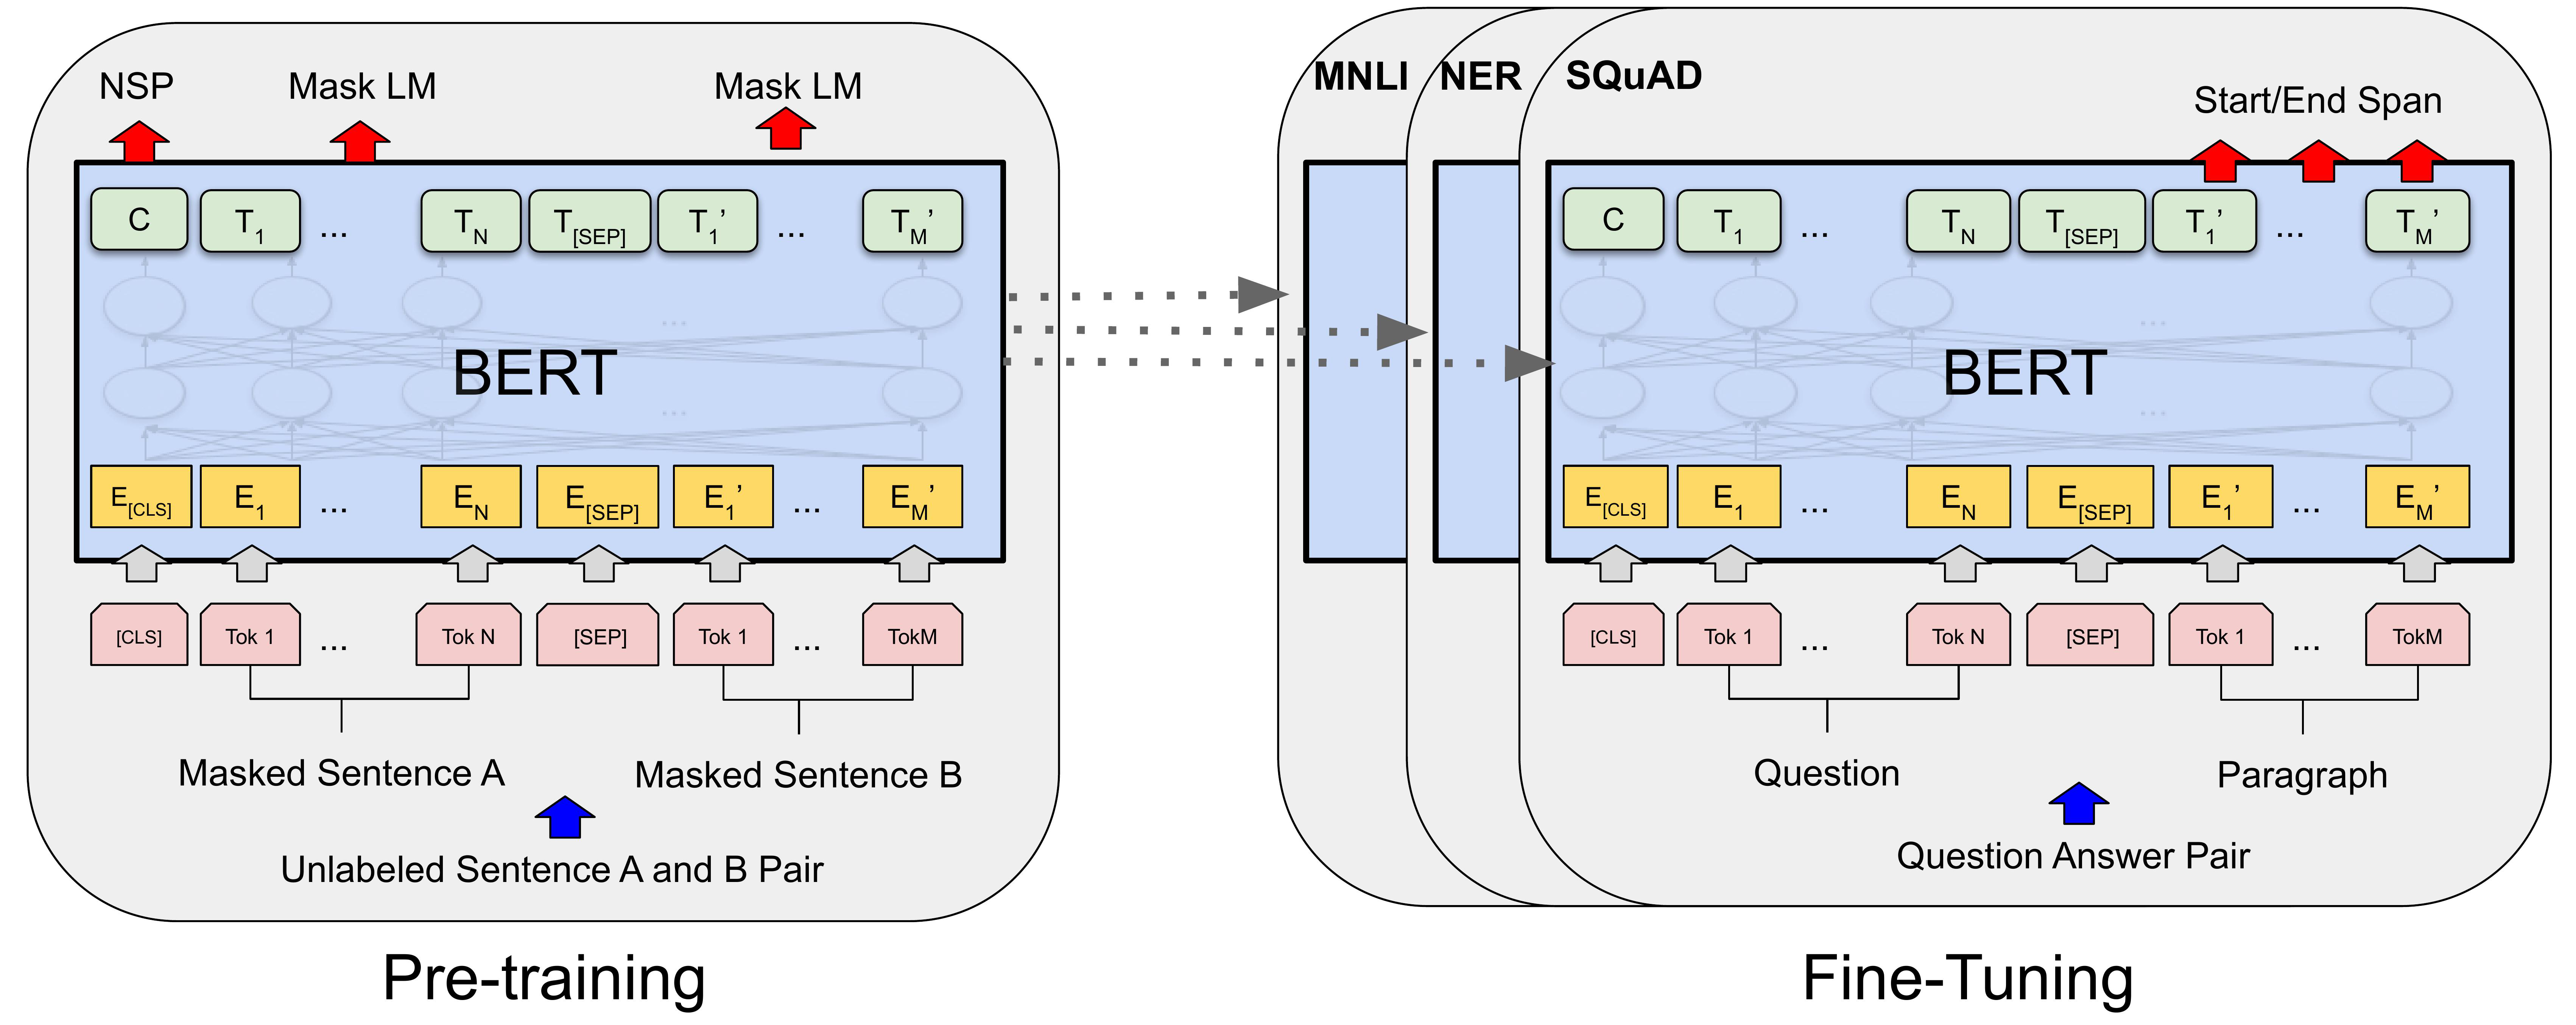
\includegraphics[width=\textwidth]{chapter-2/bert.jpg}
    \caption{Arsitektur BERT \parencite{bert}}
    \label{fig:bert}
\end{figure}

BERT merupakan \textit{pre-trained model} sehingga telah dilatih pada sejumlah besar teks. Data latih BERT diambil dari BooksCorpus dan Wikipedia bahasa Inggris \parencite{bert}. Ini memungkinkan BERT untuk mempunyai pengetahuan mendasar dalam tugas NLP. Ketika digunakan untuk tugas-tugas NLP spesifik, seperti klasifikasi teks atau pemahaman pertanyaan, BERT dapat disesuaikan dengan data tugas spesifik untuk meningkatkan kinerjanya. Seperti yang bisa dilihat pada gambar \ref{fig:bert}, BERT dilatih (\textit{pre-train}) dengan menggunakan dua tugas yaitu \textit{Masked LM} dan \textit{Next Sentence Prediction} (NSP). \textit{Masked LM} melakukan \textit{masking} pada sebagian token dan akan diprediksi oleh model BERT. Sedangkan, untuk NSP, model BERT akan menentukan mana kalimat berikutnya dari kalimat sebelumnya.

Terdapat versi bahasa Indonesia yaitu IndoBERT. IndoBERT merupakan model Transformer yang mirip dengan BERT, namun dilatih dengan bahasa Indonesia \parencite{indolem}. IndoBERT mempunyai konfigurasi yang sama dengan konfigurasi BERT, yaitu 12 \textit{layer} yang masing-masing mempunyai 768 \textit{hidden layer}, 12 \textit{attention head}, dan 3072 \textit{hidden layer} pada \textit{feed-forward layer}. IndoBERT dilatih dengan total 220 juta kata, yang didapatkan dari tiga sumber utama, yaitu Wikipedia Indonesia, sumber berita (Kompas, Tempo, dan Liputan6), dan Indonesian Web Corpus \parencite{indolem}. IndoBERT merupakan \textit{state-of-the-art} pada kakas evaluasi IndoLEM.

\subsection{\textit{Text-to-Text Transfer Transformers} (T5)}

\textit{Text-to-Text Transfer Transformers} atau biasa disebut sebagai T5 merupakan model \textit{encoder decoder} berbasis Transformer. Model ini menggunakan pendekatan \textit{text-to-text} seperti namanya, yang berarti menganggap setiap pemrosesan teks sebagai masukan dan mengeluarkannya sebagai teks juga \parencite{T5}. Dengan pendekatan ini, model T5 dapat digunakan secara langsung pada setiap tugas NLP.

\begin{figure}[ht]
    \vspace{0.25cm}
    \centering
    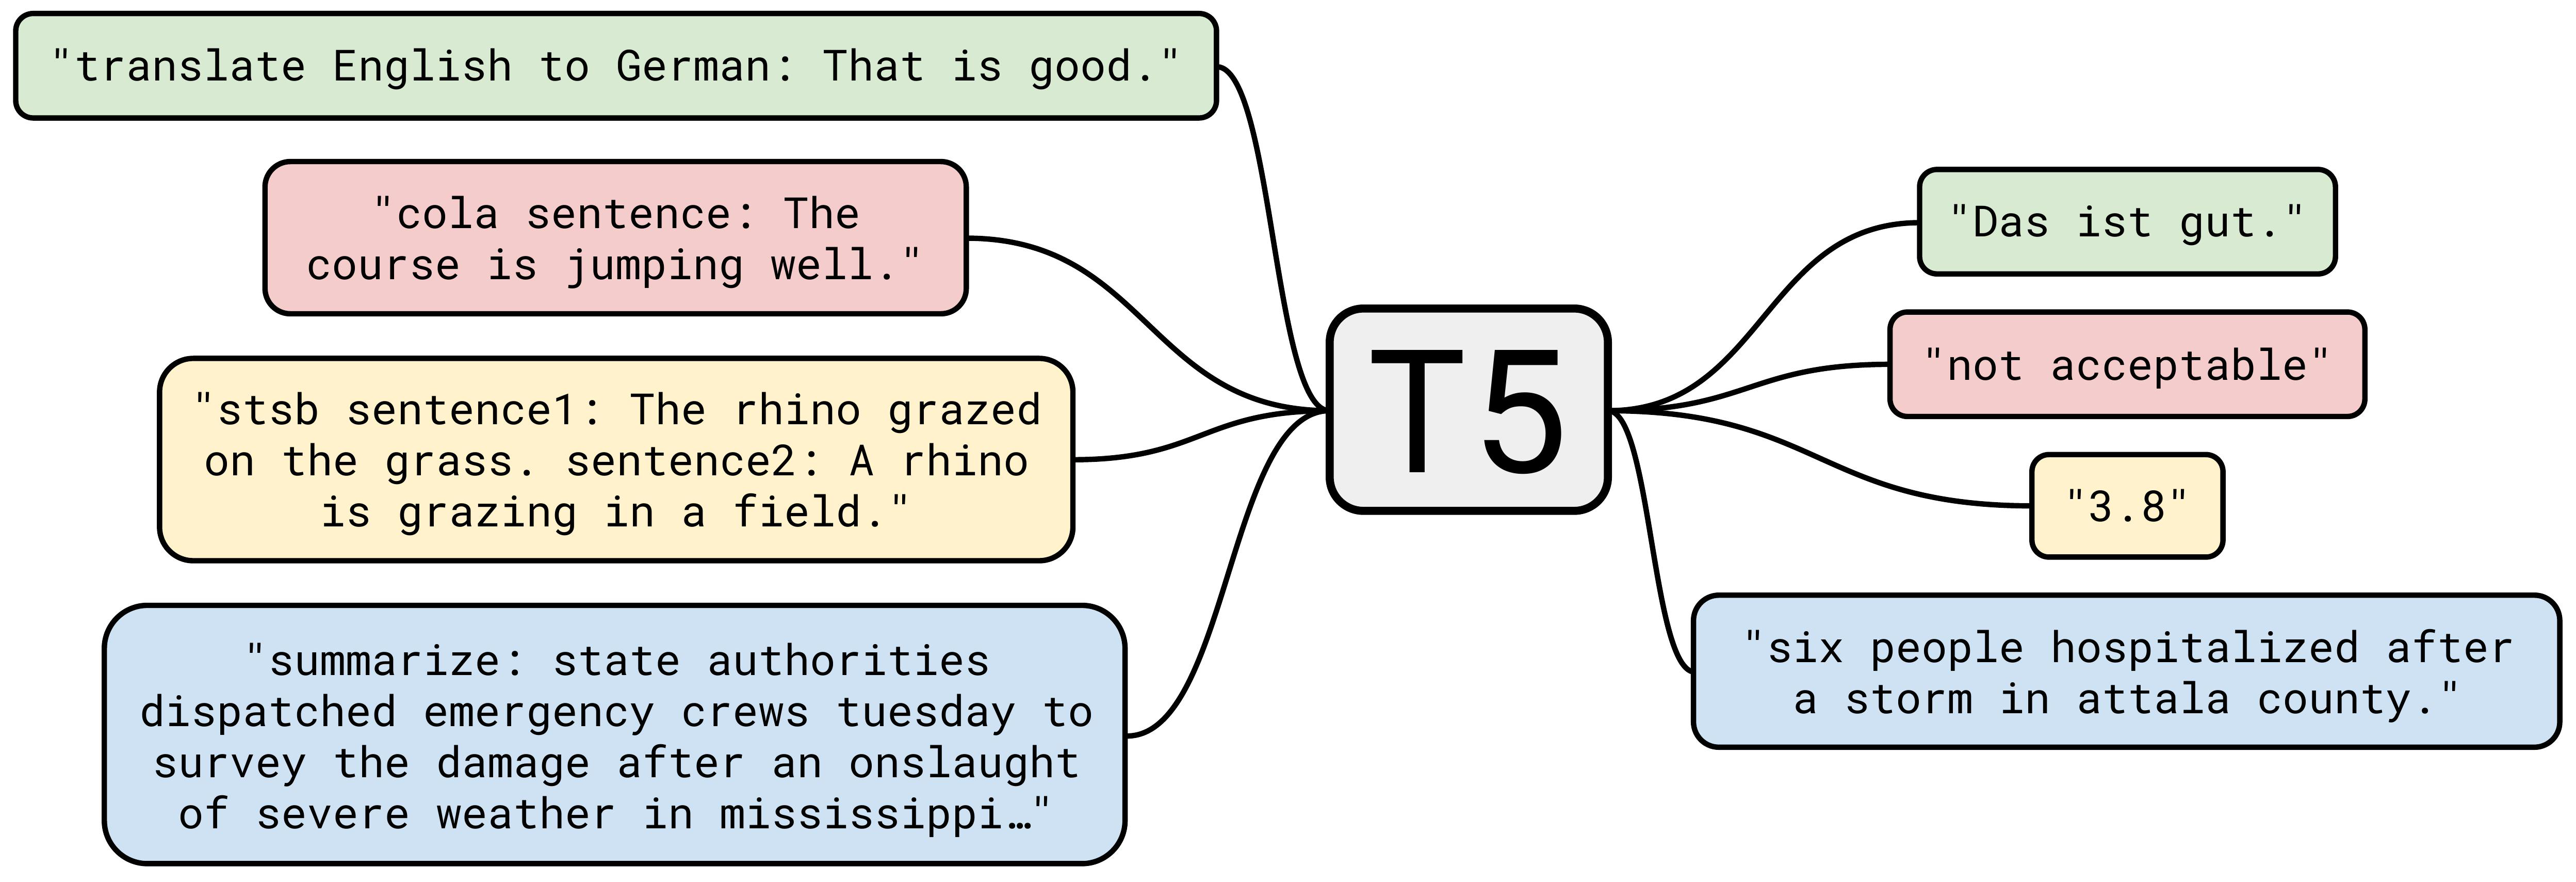
\includegraphics[width=\textwidth]{chapter-2/T5.jpg}
    \caption{\textit{Framework} dari T5 \parencite{T5}}
    \label{fig:T5}
\end{figure}

Pada gambar \ref{fig:T5}, yaitu \textit{framework} dari model T5, setiap tugas pada T5, termasuk \textit{translation, question answering}, dan \textit{classification}, semuanya akan dianggap sebagai masukan teks dan dilatih untuk menghasilkan teks lainnya lagi. T5 dilatih pada dataset \textit{Colossal Cleaned Crawled Corpus} (C4) yang merupakan koleksi dari web publik Common Crawl yang telah dibersihkan.

\begin{figure}[ht]
    \vspace{0.25cm}
    \centering
    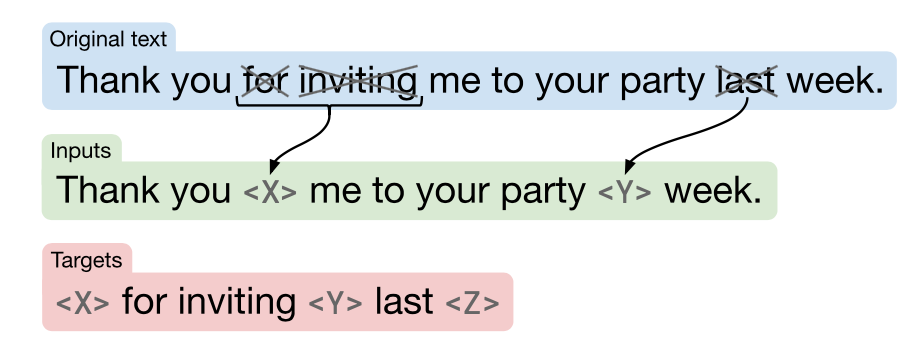
\includegraphics[width=\textwidth]{chapter-2/unsupervised_objective.png}
    \caption{\textit{Unsupervised objectives} dari T5 \parencite{T5}}
    \label{fig:unsupervised-T5}
\end{figure}

Model T5 didesain agar bagian \textit{encoder} dan \textit{decoder}-nya mirip dengan konfigurasi dari BERT \parencite{T5}. Kedua bagian tersebut terdiri dari 12 \textit{layer} yang mempunyai \textit{hidden layer, attention head}, serta \textit{feed-forward}. Mirip dengan MLLM pada BERT, model T5 dilatih \textit{pre-train} dengan menggunakan \textit{unsupervised objectives} yang bisa dilihat pada gambar \ref{fig:unsupervised-T5}. Beberapa kata yang dihilangkan secara konsekutif akan dianggap sebagai satu \textit{sentinel} token yang nantinya akan diprediksi sebagai target oleh T5.

Terdapat versi bahasa Indonesia dari T5, yaitu IndoT5. IndoT5 dilatih secara spesifik untuk bahasa Indonesia dengan menggunakan \textit{framework} pelatihan nanoT5 \parencite{indoT5}. \textit{Dataset} yang digunakan berasal dari CulturaX yang mengandung 23 juta dokumen berbahasa Indonesia. Model IndoT5 menjadi \textit{state-of-the-art} pada tugas \textit{summarization} pada kakas evaluasi IndoLEM.


\section{\textit{Parameter Efficient Fine-Tuning}}

\textit{Fine-tuning} dari \textit{pre-trained model} terbukti efektif untuk berbagai tugas NLP \parencite{fine_tuning}. Namun, melakukan \textit{fine-tuning} pada seluruh model termasuk tidak efektif secara parameter karena akan menghasilkan model baru untuk setiap tugas yang dilatih. Apalagi dengan jumlah parameter yang mencapai jutaan bahkan miliaran, model yang dihasilkan dari \textit{fine-tuning} akan sangat tidak efisisen. Banyak penelitian yang mengajukan teknik \textit{fine-tuning} yang efisien secara parameter, yaitu \PEFT dengan hanya melakukan \textit{tuning} pada sebagian dari parameter model.

\subsection{\textit{Bottleneck Adapter}}

\textit{Bottleneck adapter} merupakan modul \textit{adapter} dengan menggunakan arsitektur \textit{bottleneck} \parencite{adapter_houlsby}. Konsep \textit{bottleneck adapter} diajukan sebagai alternatif dari \textit{fine-tuning}, dengan tiga properti utama, yaitu kinerja yang baik, pelatihan yang sekuensial (tidak perlu akses secara simultan terhadap keseluruhan \textit{dataset}), dan hanya menambahkan sebagain kecil parameter untuk setiap tugas \parencite{adapter_houlsby}. Strategi \textit{fine-tuning} dengan \textit{adapter} dilakukan dengan memasukkan \textit{layer} tambahan pada arsitektur \textit{Transformer} seperti yang bisa dilihat pada gambar \ref{fig:adapters_houlsby_arch}. Seperti yang telah dibahas pada subbab \ref{sec:transformer}, setiap \textit{layer} pada \textit{Transformer} mempunyai dua \textit{sub-layer}, yaitu \textit{multi-head attention} dan \textit{feed-forward}. Metode \textit{bottleneck adapter} ini akan menambahkan modul \textit{adapter} ke setiap \textit{sub-layer} pada \textit{Transformer} tersebut \parencite{adapter_houlsby}.

\begin{figure}[h]
    \vspace{0.25cm}
    \centering
    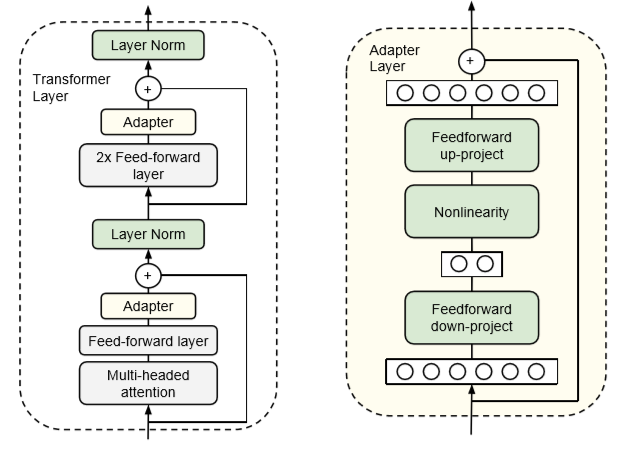
\includegraphics[width=\textwidth]{chapter-2/adapter_houlsby_arch.png}
    \caption{Arsitektur dari \textit{Bottleneck Adapter} oleh \citeauthor{adapter_houlsby} \parencite{adapter_houlsby}}
    \label{fig:adapters_houlsby_arch}
\end{figure}

Arsitektur \textit{bottleneck} dari modul \textit{adapter} diajukan untuk membatasi jumlah dari parameter \parencite{adapter_houlsby}. Berdasarkan gambar \ref{fig:adapters_houlsby_arch}, \textit{adapter} melakukan proyeksi dari dimensi asli $d$ ke dimensi yang lebih kecil $m$, lalu dilanjutkan dengan fungsi nonlinear, dan dilakukan proyeksi kembali dari dimensi $m$ ke dimensi asli $d$. Sehingga, total parameter yang ditambahkan untuk setiap \textit{layer} adalah $2md$ yang berasal dari bobot pada kedua proyeksi ditambah dengan $m+d$ yang merupakan biasnya. Pada penggunaannya, dengan memakai nilai $m << d$, parameter yang digunakan adalah sekitar $0.5-8\%$ dari parameter asli model \parencite{adapter_houlsby}.

\begin{equation}
    reduction\_factor = \frac{d_{hidden}}{d_{bottleneck}}
    \label{eq:reduction_factor}
\end{equation}

Parameter yang digunakan dibatasi dengan menggunakan $reduction\_factor$ \parencite{adapterhub}. Nilai dari $reduction\_factor$ tersebut didapat dari rasio antara dimensi asli dengan dimensi yang lebih kecil bisa dilihat pada rumus \ref{eq:reduction_factor} \parencite{adapterhub}. Nilai $d_{hidden}$ merupakan nilai dari dimensi asli $d$. Sedangkan, nilai $d_{bottleneck}$ merupakan dimensi dari \textit{bottleneck} yang lebih kecil dari dimensi aslinya.

Penggunaan \textit{adapter} tidak hanya dengan menambahkannya pada setiap \textit{sub-layer Transformer}. Terdapat beberapa konfigurasi yang bisa digunakan. Salah satunya adalah seperti pada gambar \ref{fig:adapters_houlsby_arch} oleh \parencite{adapter_houlsby} dengan menambahkan modul \textit{adapter} pada kedua \textit{sub-layer} (\textit{multi-head attention} dan \textit{feed-forward}). \citeauthor{adapter_pfeiffer} menggunakan \textit{adapter} hanya pada \textit{sub-layer feed-forward}. Sedangkan, \citeauthor{uvpl} menggunakan \textit{adapter} secara paralel pada \textit{layer transformer}.

\begin{table}[h]
    \vspace{0.25cm}
    \centering
    \caption{Hasil \textit{Adapter} konfigurasi \citeauthor{adapter_houlsby} pada GLUE \parencite{adapter_houlsby}}
    \label{table:adapter_houlsby_result}
    \resizebox{\textwidth}{!}{%
    \begin{tabular}{l|p{2cm}|p{2cm}|ccccccccc|c}
        \hline \hline
        & Total num params & Trained params / task & CoLA & SST & MRPC & STS-B & QQP & MNLI$_m$ & MNLI$_{mm}$ & QNLI & RTE & Total \\
        \hline
        BERT$_{LARGE}$ & $9.0\times$ & $100\%$ & $60.5$ & $94.9$ & $89.3$ & $87.6$ & $72.1$ & $86.7$ & $85.9$ & $91.1$ & $70.1$ & $80.4$ \\
        Adapters (8-256) & $1.3\times$ & $3.6\%$ & $59.5$ & $94.0$ & $89.5$ & $86.9$ & $71.8$ & $84.9$ & $85.1$ & $90.7$ & $71.5$ & $80.0$ \\
        Adapters (64) & $1.2\times$ & $2.1\%$ & $56.9$ & $94.2$ & $89.6$ & $87.3$ & $71.8$ & $85.3$ & $84.6$ & $91.4$ & $68.8$ & $79.6$ \\
        \hline \hline
    \end{tabular}}
\end{table}

Tabel \ref{table:adapter_houlsby_result} menunjukkan hasil evaluasi dari \textit{Adapter} dengan \textit{baseline} yang menggunakan \textit{fine-tuning} pada kakas evaluasi GLUE. \textit{Adapter} berhasil mendapatkan hasil rata-rata dengan nilai $80.0$, dibandingkan dengan \textit{fine-tuning} yang mendapatkan nilai $80.4$. Selain itu, untuk ukuran dari \textit{adapter} yang tetap yaitu dengan ukuran 64, mendapatkan hasil dengan nilai $79.6$. \textit{Adapter} mampu menyaingi kinerja \textit{fine-tuning} dengan hanya menggunakan $3.6\%$ parameter.

\subsection{\textit{Prefix-Tuning}}

\textit{Prefix-Tuning} merupakan salah satu metode PEFT yang menjadi alternatif dari metode \textit{fine-tuning} yang menggunakan vektor kontinu (disebut dengan \textit{prefix}) \parencite{prefix_tuning}. Metode ini mengambil inspirasi dari \textit{prompting}, memperbolehkan token-token berikutnya untuk memerhatikan \textit{prefix} tersebut seolah-seolah \textit{prefix} tersebut adalah \textit{virtual token} \parencite{prompt_tuning}. Mirip dengan \textit{Adapter}, \textit{prefix-tuning} hanya perlu menyimpan sedikit parameter tambahan untuk suatu tugas dengan melakukan \textit{freeze} pada parameter asli model dan hanya mengubah parameter dari \textit{prefix} tersebut.

\begin{figure}[h]
    \vspace{0.25cm}
    \centering
    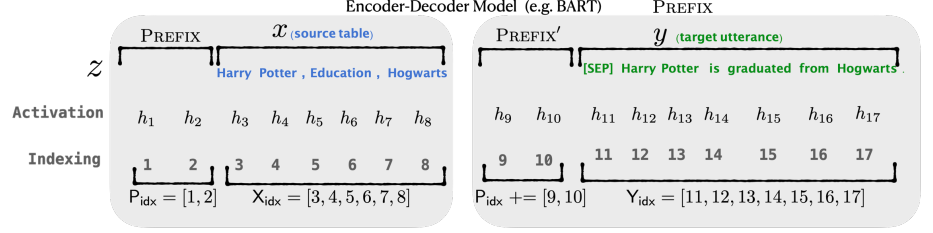
\includegraphics[width=\textwidth]{chapter-2/prefix_tuning_example.png}
    \caption{Contoh \textit{Prefix-Tuning} pada model \textit{encoder decoder} \parencite{prefix_tuning}}
    \label{fig:prefix_tuning_example}
\end{figure}

Dengan intuisi yang didapatkan dari penggunaan \textit{prompting}, penambahan konteks dapat mengarahkan model tanpa mengubah parameter \parencite{prefix_tuning}. \textit{Prefix-Tuning} menambahkan \textit{prefix} pada kedua \textit{encoder} dan \textit{decoder} untuk mendapatkan $z = [PREFIX;x;PREFIX';y]$ seperti yang bisa dilihat pada gambar \ref{fig:prefix_tuning_example}. $P_{idx}$ merupakan indeks dari \textit{prefix} tersebut. Matriks yang bisa dilatih, diinisialisasi sebagai matriks $P_\theta$ dengan $\theta$ sebagai parameternya. Dimensi dari matriks $P_\theta$ adalah panjang dari $P_{idx}$ dikalikan dengan besar dimensi \textit{activation layer}-nya yaitu $h$. Secara langsung melakukan optimisasi terhadap $P_\theta$ itu tidak stabil dan menghasilkan penurunan terhadap kinerja \parencite{prefix_tuning}. Sehingga, matriks $P_\theta$ diperamaterisasi sebagai $P_\theta = MLP_\theta(P'_\theta)$ dengan matriks dimensi lebih kecil ($P'_\theta$) dimasukkan ke dalam \textit{feed forward} ($MLP_\theta$).

\begin{figure}[h]
    \vspace{0.25cm}
    \centering
    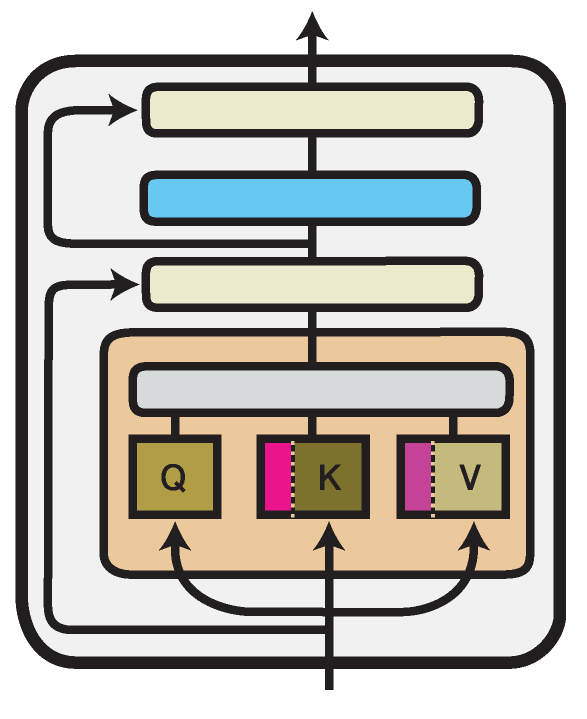
\includegraphics[height=0.4\textwidth]{chapter-2/prefix_tuning_arch.png}
    \caption{Arsitektur \textit{Prefix-Tuning} \parencite{prefix_tuning}}
    \label{fig:prefix_tuning_arch}
\end{figure}

Pada gambar \ref{fig:prefix_tuning_arch} ditunjukkan arsitektur dari \textit{Prefix-Tuning} dengan menambahkan \textit{prefix} pada \textit{multi-headattention layer}. \textit{Prefix} ditambahkan pada bagian \textit{key} dan \textit{value} pada \textit{attention head}, menjadi $P^K$ dan $P^V$. Sehingga, rumus \ref{eq:attention} akan menggunakan $[P^K, K]$ dan $[P^V, V]$ menjadi $Attention(Q, [P^K, K], [P^V, V])$ \parencite{adapterhub}. Selain itu, panjang dari \textit{prefix} dapat divariasikan berdasarkan pada nilai \textit{prefix length}-nya.

\begin{table}[h]
    \vspace{0.25cm}
    \centering
    \caption{Hasil \textit{Prefix-Tuning} pada tugas \textit{summarization} XSUM \parencite{prefix_tuning}}
    \label{table:prefix_tuning_result}
    \begin{tabular}{lccc}
        \hline
        & R-1 & R-2 & R-L \\ \hline
        FINE-TUNE & $45.14$ & $22.27$ & $37.25$ \\
        PREFIX($2\%$) & $43.80$ & $20.93$ & $36.05$ \\
        PREFIX($0.1\%$) & $42.92$ & $20.03$ & $35.05$ \\
        \hline
    \end{tabular}
\end{table}

Pada penelitian yang dilakukan oleh \citeauthor{prefix_tuning}, terdapat dua tugas yang dievaluasi yaitu \textit{table-to-text generation} dan \textit{summarization}. Seperti yang bisa dilihat pada tabel \ref{table:prefix_tuning_result}, dengan hanya $2\%$ parameter dibanding parameter aslinya, \textit{Prefix-Tuning} berhasil mendapatkan kinerja yang sedikit lebih buruk dibanding \textit{fine-tuning} ($36.05$ dibanding $37.25$ pada R-L) \parencite{prefix_tuning}. Hasil ini sedikit berbeda dibanding pada tugas \textit{table-to-text generation} yang mendapatkan hasil yang menyaingi \textit{fine-tuning}. Perbedaan antara kedua tugas tersebut adalah bahwa masukan dari artikel pada XSUM lebih banyak sekitar 17 kali dibanding pada \textit{dataset table-to-text}, serta tugas \textit{summarization} lebih kompleks dibanding \textit{table-to-text generation} karena perlu pemahaman terhadap tulisandan mengidentifikasi topik penting dari sebuah artikel \parencite{prefix_tuning}.

\subsection{\textit{Low Rank Adaptation} (LoRA)}

Konsep dasar di balik LoRA adalah ide bahwa adaptasi model untuk tugas baru tidak selalu memerlukan perubahan besar pada seluruh parameter model. Sebaliknya, perubahan kecil pada representasi tertentu dapat menghasilkan peningkatan kinerja yang signifikan. Dengan fokus pada \textit{low rank adaptation}, LoRA mengubah hanya sebagian kecil dari bobot model, sementara sebagian besar bobot lainnya tetap tidak berubah. Ini berarti bahwa hanya "sebagian" dari informasi dalam model yang diperbarui, yang mengarah pada efisiensi komputasi yang meningkat \parencite{lora}.

\begin{figure}[h]
    \vspace{0.25cm}
    \centering
    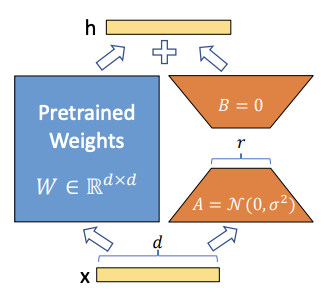
\includegraphics[width=0.8\textwidth]{chapter-2/lora.png}
    \caption{Arsitektur LoRA \parencite{lora}}
    \label{fig:lora}
\end{figure}

Salah satu kelebihan utama dari pendekatan ini adalah kemampuannya untuk mengurangi \textit{overhead} komputasi. Dalam praktiknya, ini berarti waktu \textit{training} dan sumber daya yang diperlukan untuk adaptasi model menjadi jauh lebih sedikit dibandingkan dengan metode lain yang mungkin melibatkan \textit{training} ulang model dari awal atau menambahkan sejumlah besar parameter tambahan. Arsitektur dari LoRA dapat dilihat pada Gambar \ref{fig:lora}.

Pendekatan LoRA menjadi sangat relevan, terutama saat berhadapan dengan model-model berukuran besar. Model-model seperti ini memiliki jumlah parameter yang sangat besar, sehingga \textit{training} ulang atau menambahkan parameter tambahan bisa menjadi sangat mahal dari segi komputasi. Dengan LoRA, adaptasi model-model besar menjadi lebih praktis dan dapat dilakukan dengan efisiensi yang jauh lebih tinggi, tanpa mengorbankan kinerja. Dengan demikian, LoRA menawarkan pendekatan yang menjanjikan untuk mengadaptasi \textit{pre-trained model} dengan cara yang lebih efisien.



\section{Tugas Evaluasi IndoLEM}

Dari banyaknya tugas evaluasi NLU yang tersedia, seperti GLUE, kebanyakan dari kakas tersebut hanya berfokus pada bahasa Inggris \parencite{indolem}. IndoLEM muncul untuk mengisi kekosongan tersebut dengan menyediakan tugas evaluasi yang spesifik untuk bahasa Indonesia \parencite{indolem}. IndoLEM sendiri merupakan singkatan dari \textit{Indonesian Language Evaluation Montage} (IndoLEM), dengan nama tersebut terinspirasi dari GLUE yang diterjemahkan secara langsung menjadi "LEM" \parencite{indolem}. IndoLEM menstandardisasi pembagian data dan metrik evaluasi yang digunakan, sehingga akan lebih mudah untuk direka ulang sebagai tugas evaluasi \parencite{indolem}.

Tugas evaluasi yang terdapat pada IndoLEM dibagi menjadi tiga, yaitu \textit{sequence labelling}, \textit{semantic}, dan \textit{coherency}. Untuk \textit{sequence labelling} terdapat tiga tugas, yaitu \textit{part-of-speech} (POS) \textit{tagging}, \textit{named entity recognition} (NER), dan \textit{dependency parsing}. Lalu, untuk \textit{semantic} terdapat dua tugas, yaitu \textit{sentiment analysis} dan \textit{summarization}. Terakhir, untuk \textit{coherency} terdapat dua tugas, yaitu \textit{next tweet prediction} dan \textit{tweet ordering}. Tugas yang akan dibahas pada tugas akhir ini hanya tiga, yaitu NER, \textit{sentiment analysis}, dan \textit{summarization}.

\subsection{NER pada IndoLEM}

\textit{Dataset} NER yang digunakan pada IndoLEM ada dua yaitu NER UI dan NER UGM \parencite{indolem}. Yang pertama, NER UI, terdiri dari 2.125 kalimat yang didapatkan dari anotasi yang dilakukan oleh Universitas Indonesia (UI) \parencite{indolem}. NER UGM terdiri dari 2.343 kalimat yang didapatkan dari artikel berita. NER UGM dibuat oleh Universitas Gajah Mada (UGM) \parencite{indolem}. Label pada kedua \textit{dataset} tersebut dapat dilihat pada tabel \ref{table:label-ner}. Entitas dari NER UI terdiri dari \textit{location, organization}, dan \textit{person}, sedangkan NER UGM terdiri dari 3 entitas yang sama dari NER UI ditambah \textit{quantity} dan \textit{time}.

\begin{table}[h]
    \vspace{0.25cm}
    \centering
    \caption{Label \textit{dataset} NER}
    \label{table:label-ner}
    \begin{tabular}{l|l}
        \toprule
        \multicolumn{1}{c}{\textbf{NER UI}} & \multicolumn{1}{c}{\textbf{NER UGM}} \\
        \midrule
        B-LOCATION & B-LOCATION \\
        B-ORGANIZATION & B-ORGANIZATION \\
        B-PERSON & B-PERSON \\
        - & B-QUANTITY \\
        - & B-TIME \\
        I-LOCATION & I-LOCATION \\
        I-ORGANIZATION & I-ORGANIZATION \\
        I-PERSON & I-PERSON \\
        - & I-QUANTITY \\
        - & I-TIME \\
        O & O \\
        \bottomrule
    \end{tabular}
\end{table}

Kedua \textit{dataset} dilakukan 5-\textit{fold cross validation} Kedua \textit{dataset} dilakukan 5-\textit{fold cross validation} dengan menggunakan $10\%$ sebagai validasi data \parencite{indolem}. Evaluasi yang dilakukan untuk kedua \textit{dataset} adalah \textit{entity-level} F1 yang dilakukan pada data tes. Selain itu, \citeauthor{indolem} melakukan evaluasi terhadap kedua \textit{dataset} tersebut dan ditemukan bahwa kualitas NER UI lebih baik dibandingkan NER UGM, dengan kesalahan pada NER UGM sebagian besar karena rendahnya nilai \textit{recall}, yaitu memberikan label O pada entitas bernama \parencite{indolem}.

\begin{table}[h]
    \vspace{0.25cm}
    \centering
    \caption{Hasil evaluasi NER pada IndoLEM}
    \label{table:indolem-ner-result}
    \begin{tabular}{lcc}
        \toprule
        \textbf{Method} & \textbf{NER UGM F1} & \textbf{NER UI F1} \\
        \midrule
        BiLSTM-CRF & 70,9 & 82,2 \\
        mBERT & 71,6 & 82,2 \\
        MALAYBERT & 73,2 & 87,4 \\
        INDOBERT & \textbf{74,9} & \textbf{90,1} \\
        \bottomrule 
    \end{tabular}
\end{table}

Hasil evaluasi dapat dilihat pada tabel \ref{table:indolem-ner-result}, dengan \textit{baseline} merupakan BiLSTM dengan 300d \texttt{fastText} \textit{embedding} berbahasa Indonesia \parencite{indolem}. Untuk model BERT dilakukan metode \textit{fine-tuning} dengan nilai $learning\_rate$ yaitu $5e-5$ dan dilakukan dengan 100 $epoch$. IndoBERT mendapatkan nilai terbaik untuk kedua \textit{dataset}.

\subsection{\textit{Sentiment Analysis} pada IndoLEM}

\textit{Dataset sentiment analysis} pada IndoLEM berasal dari Twitter dan ulasan hotel \parencite{indolem}. Data ulasan hotel berisi sentimen pada level aspek, dengan setiap ulasan mempunyai beberapa polaritas pada aspek yang berbeda \parencite{indolem}. Dilakukan perhitungan proporsi antara aspek positif dan negatif, dan label diberikan kepada aspek yang merupakan mayoritas \parencite{indolem}. \textit{Sentiment analysis} yang dilakukan pada IndoLEM menggunakan klasifikasi biner, label 0 berarti negatif dan sebaliknya. Pembagian \textit{dataset} adalah 3638 untuk data pelatihan, 399 untuk data evaluasi, dan 1011 untuk data tes \parencite{indolem}. 

\begin{table}[h]
    \vspace{0.25cm}
    \centering
    \caption{Hasil evaluasi \textit{sentiment analysis} pada IndoLEM}
    \label{table:indolem-sentiment-result}
    \begin{tabular}{lc}
        \toprule
        \textbf{Method} & \textbf{Sentiment Analysis (F1)} \\
        \midrule
        Naive Bayes & 70,95 \\
        Logistic Regression & 72,14 \\
        BiLSTM w/ \texttt{fastText} & 71,62 \\
        mBERT & 76,58 \\
        MALAYBERT & 82,02 \\
        INDOBERT & \textbf{84,13} \\
        \bottomrule
    \end{tabular}
\end{table}

\textit{Dataset} tersebut juga dilakukan 5-\textit{fold cross validation} karena data yang tidak seimbang dan \textit{low-resource} \parencite{indolem}. Metrik evaluasi yang digunakan adalah skor F1. Evaluasi dilakukan dengan \textit{baseline} yaitu BiLSTM, Naive Bayes, dan \textit{logistic regression}. Setiap model BERT menggunakan masukan sebanyak 200 token, $learning\_rate$ dengan nilai $5e-5$, $batch\_size$ dengan nilai 30, dan $warm\_up$ sebesar $10\%$ dari total $step$. Berdasarkan tabel \ref{table:indolem-sentiment-result}, IndoBERT juga mendapatkan nilai terbaik untuk tugas evaluasi \textit{sentiment analysis}.

\subsection{\textit{Summarization} pada IndoLEM}

\begin{table}[h]
    \caption{Data \textit{summarization}}
    \label{table:label-summarization}
    \begin{center}
        \begin{tabular}{l|l}
            \toprule
            \textbf{Objek} & \textbf{Deskripsi} \\
            \midrule
            id & nilai unik untuk setiap artikel \\
            paragraphs & \textit{list} dari paragraf yang berasal dari artikel \\
            summary & ringkasan dari artikel, disimpan sebagai \textit{list} dari kalimat \\ 
            gold\_labels & label ekstraktif dari setiap kalimat pada artikel \\
            category & kategori dari artikel \\
            source & sumber artikel \\
            source\_url & URL dari artikel \\
            \bottomrule
        \end{tabular}
    \end{center}
\end{table}

Tugas \textit{summarization} menggunakan \textit{dataset} yang telah tersedia yaitu IndoSUM \parencite{summarization}. IndoSUM berisi sekitar 19.000 dokumen-ringkasan \textit{dataset} \parencite{indolem}, dengan setiap dokumen mempunyai satu \textit{abstractive summary}. \citeauthor{summarization} merilis IndoSUM beserta dengan ORACLE, yaitu sekumpulan \textit{extractive summary} yang dihasilkan secara otomatis dengan memaksimalkan skor ROUGE antar kalimat pada dokumen dengan \textit{abstractive summary}-nya \parencite{indolem}. Label pada \textit{dataset} IndoSUM dapat dilihat pada tabel \ref{table:label-summarization}.

\begin{table}[h]
    \vspace{0.25cm}
    \centering
    \caption{Hasil evaluasi \textit{summarization} pada IndoLEM}
    \label{table:indolem-summarization-result}
    \begin{tabular}{lccc}
        \toprule
        \textbf{Method} & \textbf{R1} & \textbf{R2} & \textbf{RL} \\
        \midrule
        \textsc{Oracle} & 79,27 & 72,52 & 78,82 \\
        Kurniawan and Louvan (2018) & 17,62 & 4,70 & 15,89 \\
        Cheng and Lapata (2016) & 67,96 & 61,65 & 67,24 \\
        mBERT & 68,40 & 61,66 & 67,67 \\
        MALAYBERT & 68,44 & 61,38 & 67,71 \\
        INDOBERT & \textbf{69,93} & \textbf{62,86} & \textbf{69,21} \\
        \bottomrule
    \end{tabular}
\end{table}

\textit{Dataset} ini juga dilakukan 5-\textit{fold cross validation}. Evaluasi dilakukan dengan menggunakan dua \textit{baseline}, yaitu \citeauthor{summarization} dan \citeauthor{summarization_lstm} beserta ORACLE yang merupakan batas atas dari \textit{extractive summary}. Untuk model BERT mengikuti penelitian dari \citeauthor{summarization_bert} \parencite{indolem}. Metrik evaluasi yang digunakan adalah skor ROUGE, yaitu R1, R2, dan RL. Hasil evaluasi dapat dilihat pada tabel \ref{table:indolem-summarization-result}, dengan IndoBERT mendapatkan nilai yang terbaik juga.


\section{Metrik Evaluasi}

Dalam proses \textit{training} model, diperlukan metode evaluasi sebagai penilaian kinerja model dengan membandingkan metrik yang dihasilkan oleh model tersebut. Metrik ini digunakan pada model klasifikasi dengan membandingkan hasil prediksi dengan target aslinya. Hasil prediksi ini dapat direpresentasikan sebagai \textit{confusion matrix}. Berdasarkan \citeauthor{metrics}, terdapat beberapa metrik yang dapat dihasilkan berdasarkan \textit{confusion matrix}, yaitu \textit{accuracy}, \textit{precision}, \textit{recall}, dan F1-\textit{Score}.

\begin{table}[ht]
    \vspace{0.25cm}
    \centering
    \caption{Tabel \textit{confusion matrix} \parencite{metrics}}
    \label{table:confusion-matrix}
    \begin{tabular}{l|c|c}
        \toprule
        \multicolumn{1}{c|}{\textbf{Target}} & \multicolumn{2}{c}{\textbf{Prediksi}} \\
        & \textbf{Positif} & \textbf{Negatif} \\
        \midrule
        \textbf{Positif} & \textit{True Positive} (TP) & \textit{False Negative} (FN) \\
        \textbf{Negatif} & \textit{False Positive} (FP) & \textit{True Negative} (TN) \\
        \bottomrule
    \end{tabular}
\end{table}

Berdasarkan tabel \ref{table:confusion-matrix} terdapat empat hasil prediksi. \textit{True Positive} (TP) yang berarti model memprediksi kelas positif yang memang bernilai positif sesuai kelasnya. True Negative (TN) memprediksi kelas negatif dan kelas tersebut memang bernilai negatif. Sedangkan, \textit{False Positive} (FP) me\textit{mprediksi kelas} positif, tetapi kelas tersebut bernilai negatif. Sebaliknya juga untuk \textit{False Negative} (FN), model memprediksi kelas tersebut sebagai negatif, tetapi kelas tersebut bernilai positif.

\subsection{\textit{Accuracy, Precision}, dan \textit{Recall}}
Nilai \textit{accuracy} dihitung sebagai proporsi hasil prediksi yang benar (baik TP maupun TN) dari total jumlah prediksi \parencite{metrics}. Metrik ini memberikan gambaran keseluruhan tentang keefektifan model. Rumus untuk menghitung nilai \textit{accuracy} dapat dilihat pada rumus \ref{eq:accuracy} \parencite{metrics}.

\begin{equation}
    Accuracy = \frac{TP + TN}{TP + TN + FP + FN}
    \label{eq:accuracy}
\end{equation}

Nilai \textit{precision} dihitung sebagai proporsi hasil prediksi kelas positif yang benar dengan jumlah kelas positif yang diprediksi, rumus untuk menghitung nilai ini dapat bisa dilihat pada rumus \ref{eq:precision} \parencite{metrics}. Sedangkan, nilai \textit{recall} dihitung sebagai proporsi antara hasil prediksi kelas positif yang benar dengan jumlah kelas positif aslinya, perhitungannya bisa dilihat pada rumus \ref{eq:recall} \parencite{metrics}.

\begin{equation}
    Precision = \frac{TP}{TP + FP}
    \label{eq:precision}
\end{equation}
\begin{equation}
    Recall = \frac{TP}{TP + FN}
    \label{eq:recall}
\end{equation}

\subsection{F1-\textit{Score}}
Nilai F1-\textit{Score} direpresentasikan sebagai nilai rata-rata harmonis dari nilai \textit{precision} dan \textit{recall}, bisa dilihat pada rumus \ref{eq:f1-score} \parencite{metrics}. Metrik ini berfungsi untuk mengukur keseimbangan dari kedua metrik tersebut.

\begin{equation}
    F1-Score = 2 \times \frac{Precision \times Recall}{Precision + Recall}
    \label{eq:f1-score}
\end{equation}

Terdapat beberapa jenis perhitungan untuk skor F1, yaitu \textit{micro, macro}, dan \textit{weighted}. \textit{Micro} F1 dihitung dengan nilai masing-masing \textit{precision} dan \textit{recall} secara global. Sedangkan, \textit{macro} F1 dihitung dengan rata-rata dari nilai F1 pada masing-masing kelasnya. Lalu, untuk \textit{weighted} F1 mirip seperti \textit{macro} dengan tambahan perhitungan bobot untuk setiap kelasnya berdasarkan banyak data pada kelas tersebut.

\subsection{ROUGE \textit{Score}}

ROUGE merupakan singkatan dari \textit{Recall-Oriented Understudy for Gisting Evaluation}. ROUGE biasa digunakan untuk tugas seperti \textit{summarization} dan juga translasi teks \parencite{rouge}. Evaluasi manual oleh manusia dengan membandingkan beberapa jenis aspek (koherensi, gramatikal, dan konten) akan memakan waktu yang banyak \parencite{rouge}. Sehingga, evaluasi secara otomatis terdapat tugas tersebut dibutuhkan, oleh karena itu ROUGE diajukan sebagai metode evaluasi otomatis \parencite{rouge}.

ROUGE mengukur kemampuan dari sebuah model dalam memprediksi kata-kata yang muncul pada target dari hasil prediksi, pada konteks ini adalah hasil ringkasan atau translasi teks. Terdapat beberapa jenis evaluasi ROUGE, salah satunya adalah ROUGE-N dan ROUGE-L. ROUGE-N mengukur banyaknya n-\textit{gram} kata-kata dibandingkan dengan targetnya, sebagai contoh ROUGE-1 berarti mengukur banyaknya 1 kata \parencite{rouge}. Sedangkan, ROUGE-L menggunakan \textit{Lowest Common Subsequence} (LCS) yang mengidentifikasi urutan kata terpanjang secara berurutan dalam hasil prediksi dibandingkan dengan targetnya \parencite{rouge}.


\section{Penelitian Terkait}

Penelitian yang dilakukan oleh \citeauthor{peft_on_plm} membandingkan secara komprehensif terkait metode \textit{transfer-learning} yang efisien secara parameter pada \textit{pre-trained model}. Metode ini disebut sebagai \textit{delta-tuning} pada penelitian tersebut, dengan kata 'delta' muncul dari notasi matematika yang merepresentasikan perubahan \parencite{peft_on_plm}. Metode \textit{delta-tuning} yang digunakan adalah \textit{prompt-tuning} (PT), \textit{prefix-tuning} (PF), LoRA (LR), dan \textit{adapter} (AP). \textit{Delta-tuning} tersebut  dibandingkan dengan \textit{fine-tuning} (FT) .

Eksperimen yang dilakukan pada penelitian tersebut dilakukan pada model T5 dengan konfigurasi BASE dan LARGE. Evaluasi metode \textit{delta-tuning} pada model T5 dilakukan pada 100 tugas pemrosesan bahasa alami yang diambil dari \textit{dataset} Huggingface. Tugas yang dipilih termasuk \textit{text classification}, \textit{question answering}, dan \textit{generation}.

Berdasarkan hasil yang didapatkan pada eksperimen tersebut, metode \textit{delta-tuning} dengan pengurangan jumlah parameter yang dilatih dibandingkan dengan \textit{fine-tuning} memberikan hasil yang hampir setara pada sebagian besar tugas. Metode \textit{prefix-tuning}, LoRA, dan \textit{adapter} secara kinerja hampir mirip antara satu sama lain. Bahkan, metode \textit{delta-tuning} pada sebagian tugas mampu memberikan hasil yang dominan dibanding \textit{fine-tuning}. Secara keseluruhan, kinerja pada setiap metode dapat diurutkan sebagai berikut.

\begin{enumerate}
    \item \textit{Fine-Tuning} (FT)
    \item \textit{Low-Rank Adaptation} (LoRA)
    \item \textit{Adapter Tuning} (AP)
    \item \textit{Prefix Tuning} (PF)
    \item \textit{Prompt Tuning} (PT)
\end{enumerate}

\begin{figure}[ht]
    \centering
    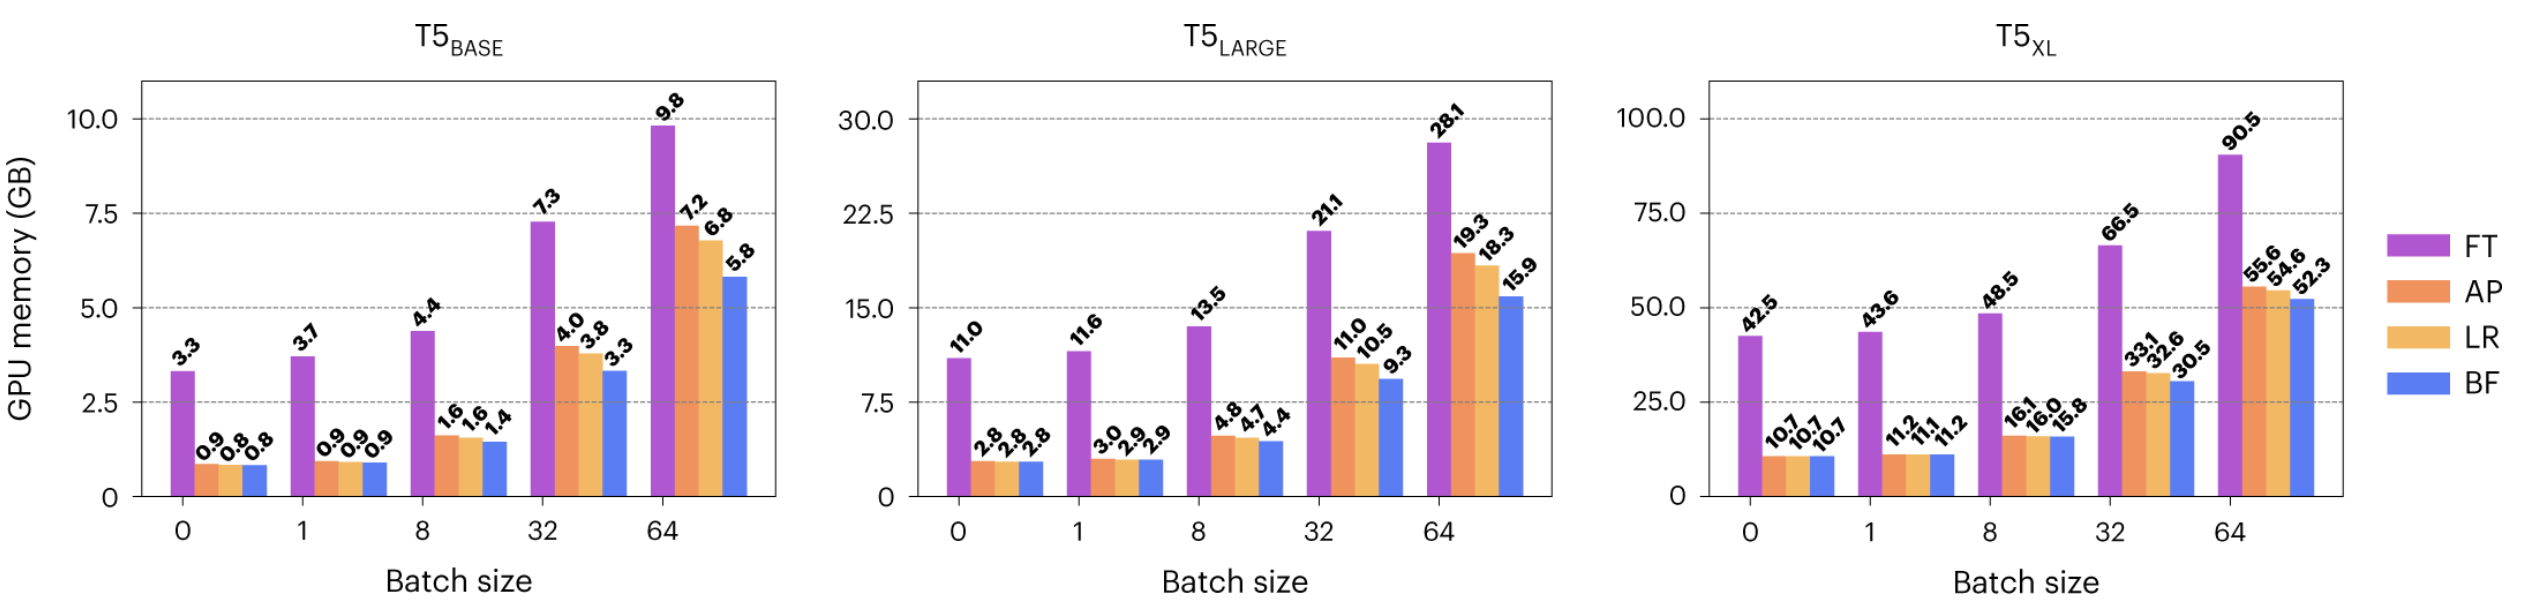
\includegraphics[width=1\textwidth]{chapter-2/peft_on_plm_memory.png}
    \caption{Perbandingan Efisiensi Memori \parencite{peft_on_plm}}
    \label{fig:peft_on_plm_memory}
\end{figure}

Selain itu, dilakukan juga eksperimen terkait analisis pada efisiensi dari tiap metode. Eksperimen ini mengeksplorasi penggunaan efisiensi memori GPU pada metode \textit{delta-tuning} dan FT pada model T5 dengan konfigurasi BASE, LARGE, dan XL. Metode \textit{delta-tuning} yang digunakan adalah LoRA (LR), dan \textit{adapter} (AP), dan BitFit (BF). Berdasarkan Gambar \ref{fig:peft_on_plm_memory}, penggunaan memori pada setiap metode \textit{delta-tuning} berkurang dibandingkan dengan \textit{fine-tuning}. Hasil ini menunjukkan bahwa \textit{delta-tuning} mengurangi penggunaan memori GPU dengan mengurangi kebutuhan komputasi gradien untuk mengubah parameter \parencite{peft_on_plm}.



\section{Kakas Pengembangan}

Pada tugas akhir ini terdapat beberapa kakas yang digunakan untuk memanfaatkan metode PEFT pada tugas evaluasi IndoLEM, kakas tersebut yaitu Transformers dari Huggingface dan Adapters. Pada subbab ini dijelaskan mengenai masing-masing kakas tersebut.

\subsection{Transformers}

Transformers merupakan pustaka kolektif (\textit{open-source}) yang diinisialisasi oleh Huggingface. Transformers berfungsi sebagai pustaka yang dapat diakses secara umum terkait dengan arsitektur Transformer \parencite{huggingface}. Pustaka ini berisi berbagai macam \textit{pre-trained model} berbasis arsitektur Transformer yang dapat digunakan melalui pustaka tersebut, sehingga memudahkan pengguna untuk memakai model \parencite{huggingface}.

\begin{figure}[h]
    \vspace{0.25cm}
    \centering
    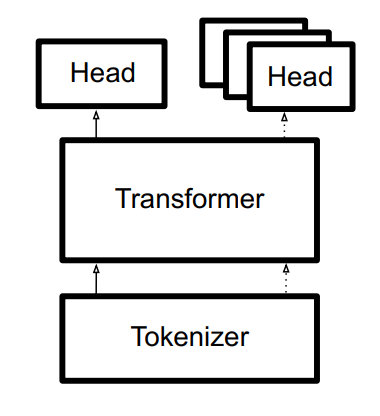
\includegraphics[width=0.6\textwidth]{chapter-2/huggingface.png}
    \caption{Komponen dari Model pada Transformers \parencite{huggingface}}
    \label{fig:huggingface}
\end{figure}

Setiap model pada pustaka Transformers terdiri dari tiga komponen yaitu, Tokenizer, Transformer, dan Head, seperti yang bisa dilihat pada gambar \ref{fig:huggingface} \parencite{huggingface}. Komponnen Tokenizer berfungsi untuk melakukan tokenisasi atau melakukan konversi dari teks asli ke sebuah \textit{enconding} \parencite{huggingface}. Lalu, komponen Transformer melanjutkan hasil dari Tokenizer tersebut, yaitu mengubah \textit{encoding} menjadi \textit{contextual embedding} \parencite{huggingface}. Terakhir, komponen Head akan mengubah \textit{contextual embedding} dari komponen Transformer menjadi sebuah prediksi yang spesifik kepada tugas evaluasi yang sedang dilatih \parencite{huggingface}.

\begin{table}[h]
    \caption{Contoh kode penggunaan Transformers}
    \label{table:huggingface-model-code}
    \begin{lstlisting}[language=python]
    tknzr = AutoTokenizer.from_pretrained("bert-base-uncased")
    model = AutoModel.from_pretrained("bert-base-uncased")
    \end{lstlisting}
\end{table}

Tabel \ref{table:huggingface-model-code} adalah contoh pemanggilan model dengan menggunakan Transformers. \texttt{AutoTokenizer} merupakan komponen Tokenizer yang berfungsi sebagai tokenisasi dan \texttt{AutoModel} merupakan komponen Transformer sebagai \textit{pre-trained model} yang digunakan. Komponen Head dapat ditambahkan dengan menambahkan tugas evaluasi spesifik di belakang pemanggilan model, sebagai contoh untuk tugas klasifikasi akan ditambahkan \texttt{ForSequenceClassification} pada model, sehingga menjadi \texttt{AutoModelForSequenceClassification}.

\begin{table}[h]
    \caption{Argumen pada modul Trainer}
    \label{table:huggingface-trainer-code}
    \begin{lstlisting}[language=python]
    (
        model: Union = None,
        args: TrainingArguments = None,
        data_collator: Optional = None,
        train_dataset: Union = None,
        eval_dataset: Union = None,
        tokenizer: Optional = None,
        model_init: Optional = None,
        compute_metrics: Optional = None,
        callbacks: Optional = None,
        optimizers: Tuple = (None, None),
        preprocess_logits_for_metrics: Optional = None
    )
    \end{lstlisting}
\end{table}

Pustaka Transformers juga menyediakan modul Trainer yang berfungsi untuk pelatihan model. Pelatihan ini dilakukan dengan menggunakan pustaka PyTorch, sehingga mampu menggunakan CUDA yang berfungsi untuk melatih model secara paralel. Argumen yang digunakan pada modul Trainer dapat dilihat pada tabel \ref{table:huggingface-trainer-code}. \textit{Hyperparameter} untuk pelatihan dapat diatur dari model \texttt{TrainingArguments}.

Modul lain yang umum digunakan adalah HfArgumentParser yang berfungsi untuk melakukan \textit{parsing} terhadap argumen yang digunakan. Modul ini akan membaca argumen yang diberikan oleh pengguna melalui \textit{script}, lalu hasil pembacaan tersebut dapat digunakan. Argumen yang diterima bukan hanya argumen untuk pelatihan (\textit{hyperparameter}), dapat dibuat kelas untuk melakukan \textit{parsing} terhadap argumen lain, salah satunya adalah untuk \textit{dataset}. Untuk dokumentasi yang lengkap terkait pustaka Transformers dapat dilihat pada tautan berikut \url{https://huggingface.co/docs/transformers}.

\subsection{Adapters}

Adapters merupakan pustaka kolektif (\textit{open-source}) yang diinisialisasi oleh \citeauthor{adapters}. Pustaka Adapters merupakan penyatuan dari berbagai metode PEFT \parencite{adapters}. Terdapat beberapa metode PEFT yang diimplementasikan pada pustaka tersebut salah satunya adalah \textit{Adapter}, \textit{Prefix-Tuning}, LoRA, IA3, dan lain-lain. Metode PEFT yang tersedia beserta konfigurasi penggunaannya dapat dilihat pada tabel \ref{table:adapters-method}. 

\begin{table}[h]
    \vspace{0.25cm}
    \centering
    \caption{Metode PEFT pada pustaka Adapters dan konfigurasinya \parencite{adapters}}
    \label{table:adapters-method}
    \begin{tabular}{ll}
        \toprule
        \textbf{Method Name} & \textbf{Default Config} \\
        \midrule
        Bottleneck adapter \parencite{adapter_houlsby} & \texttt{[double\_]seq\_bn} \\
        Invertible adapter \parencite{adapter_pfeiffer} & \texttt{seq\_bn\_inv} \\
        Prompt tuning \parencite{prompt_tuning} & \texttt{prompt\_tuning} \\
        Prefix tuning \parencite{prefix_tuning} & \texttt{prefix\_tuning} \\
        Compacter \parencite{compacter} & \texttt{compacter} \\
        LoRA \parencite{lora} & \texttt{lora} \\
        (IA)$^3$ \parencite{ia3} & \texttt{ia3} \\
        Parallel adapter \parencite{uvpl} & \texttt{par\_bn} \\
        Mix-and-Match adapter \parencite{uvpl} & \texttt{mam} \\
        UniPELT \parencite{unipelt} & \texttt{unipelt} \\
        \bottomrule
    \end{tabular}
\end{table}

Adapters merupakan penelitian selanjutnya dari AdapterHub yang merupakan \textit{fork} dari pustaka Transformers \parencite{adapters}. Sehingga, implementasinya didasarkan pada kode yang termuat pada pustaka Transformers. Pustaka Adapters menawarkan integrasi dengan pustaka Transformers, \textit{script} adaptasi untuk penggunaan metode PEFT, dan juga fungsionalitas untuk menyimpan dan memuat metode PEFT yang telah dilatih \parencite{adapters}.

\begin{table}[h]
    \caption{Contoh kode penggunaan Adapters}
    \label{table:adapters-code}
    \begin{lstlisting}[language=python]
    import adapters
    from transformers import AutoModel
    model = AutoModel.from_pretrained("..")
    adapters.init(model)
    model.add_adapter("a", config="seq_bn")
    model.add_adapter("b", config="seq_bn")
    model.train_adapter(Parallel("a", "b"))
    \end{lstlisting}
\end{table}

Tabel \ref{table:adapters-code} menunjukkan contoh kode untuk penggunaan metode PEFT pada pustaka Adapters. Metode PEFT diinisialisasi dengan menggunakan fungsi \texttt{init}, lalu ditambahkan dengan \texttt{add\_adapter}. Untuk melatih metode PEFT, sehingga hanya melatih parameter dari metode PEFT tersebut (\textit{freeze} pada parameter asli model), perlu dilakukan pemanggilan pada fungsi \texttt{train\_adapter}. Model tidak harus diinisialisasi dengan menggunakan fungsi \texttt{init}, melainkan dapat diinisialisasi dengan memanggil \texttt{XXXAdapterModel} yang mirip dengan penggunaan pada Transformers. Sebagai contoh, \texttt{XXXAdapterModel} dapat digunakan dengan memanggil \texttt{AutoAdapterModel}. Modul Trainer juga terdapat ekuivalen untuk PEFT-nya yaitu AdapterTrainer. Begitu pula dengan TrainingArgument, terdapat AdapterArguments sebagai \textit{hyperparameter} dari metode PEFT. Untuk dokumentasi yang lengkap terkait pustaka Adapters dapat dilihat pada tautan berikut \url{https://docs.adapterhub.ml/}.

